\begin{frame}
  \frametitle{Simple vs. complex settings - QITL-01 revisited}

  \begin{itemize}

  \item  Arppe \& J{\"a}rvikivi (2002, 2007)

  \item \textit{Person} (FIRST PERSON SINGULAR or not) and
    \textit{Countability} (COLLECTIVE or not) of AGENT/SUBJECT of
    Finnish verb synonym pair \textit{mietti{\"a}} vs. \textit{pohtia}
    'think, ponder': \\

{\tiny
\begin{table}[h]
\begin{tabular}{ c  c || c || c  c}
\hline
Forced-choice                         &                 & Frequency           &                                       & Acceptability    \\
Dispreferred                          & Preferred       & (relative)          & Unacceptable                          & Acceptable       \\ \hline \hline
\multicolumn{1}{c|}{$\varnothing$}    & mietti{\"a}+SG1 & Frequent            & \multicolumn{1}{c|}{$\varnothing$}    & mietti{\"a}+SG1  \\
\multicolumn{1}{c|}{}                 & pohtia+COLL     &                     & \multicolumn{1}{c|}{}                 & pohtia{\"a}+COLL \\ \hline
\multicolumn{1}{c|}{mietti{\"a}+COLL} &                 &                     & \multicolumn{1}{c|}{}                 &                  \\
\multicolumn{1}{c|}{pohtia+SG1}       & $\varnothing$   & Rare                & \multicolumn{1}{c|}{mietti{\"a}+COLL} & pohtia+SG1       \\
\hline
\end{tabular}
\end{table}
}

  \end{itemize}
\end{frame}

\begin{frame}
  \frametitle{QITL-1 through the lenses of NDL: 2/4}

  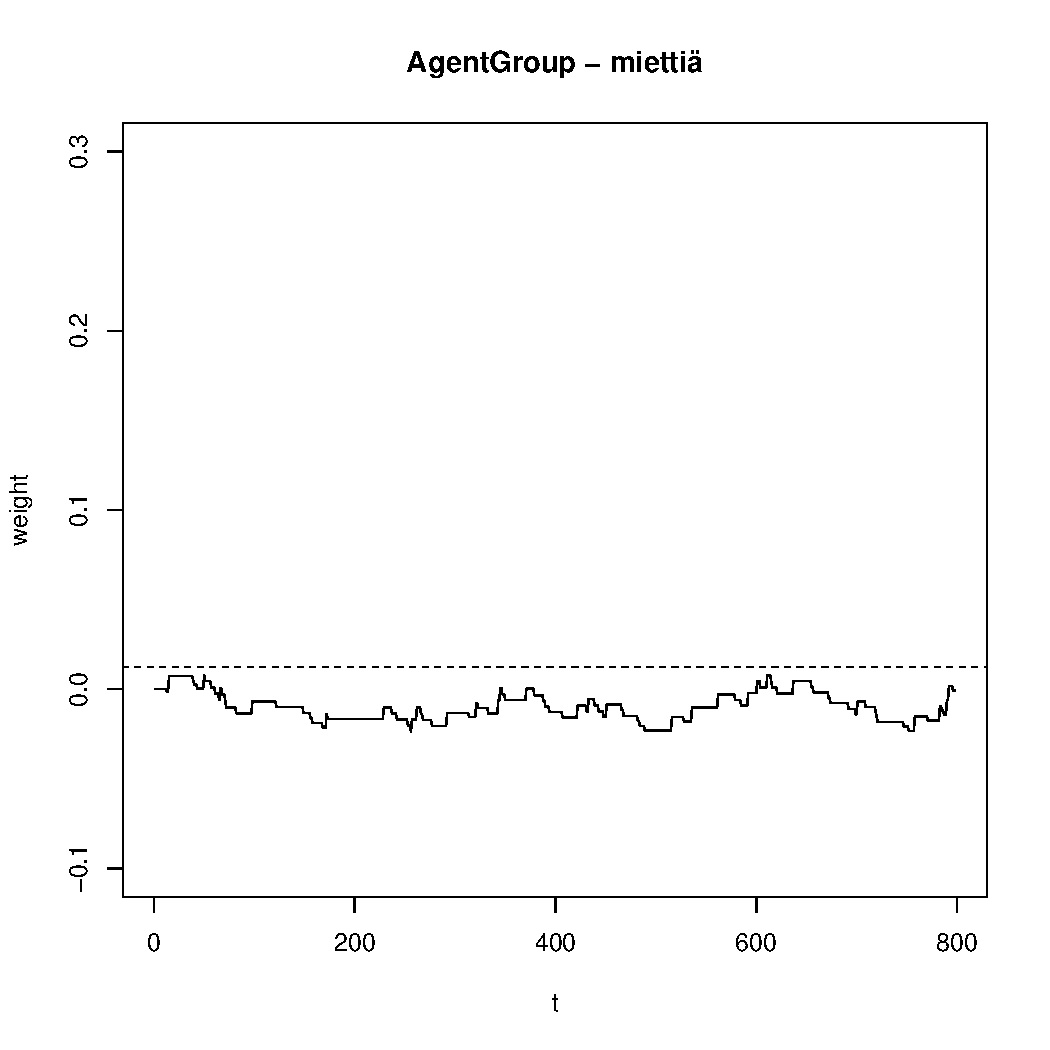
\includegraphics[width=8cm]{{{img/think.qitl1.AgentGroup_miettia_RW_vs_D}}}
  
\end{frame}

\begin{frame}
  \frametitle{QITL-1 through the lenses of NDL: 3/4}

  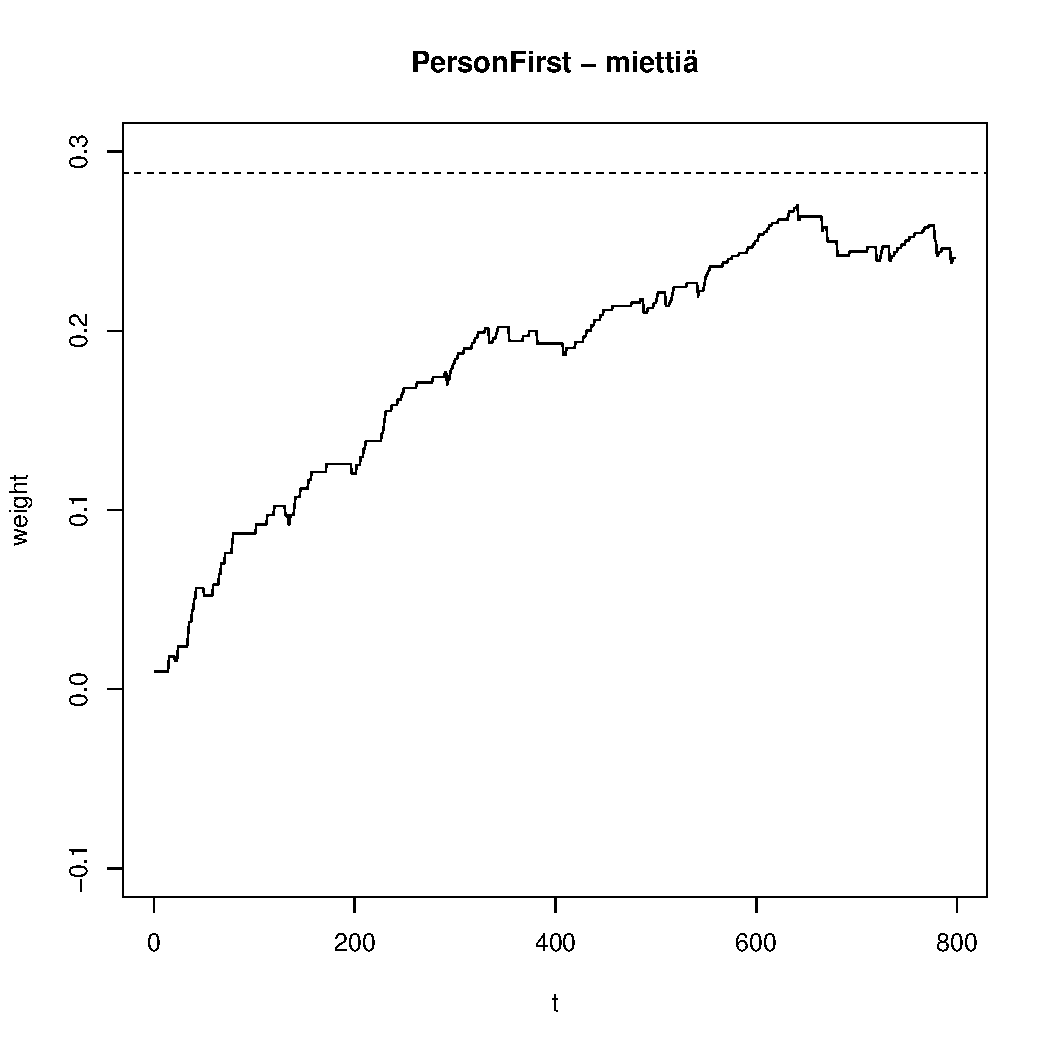
\includegraphics[width=8cm]{{{img/think.qitl1.PersonFirst_miettia_RW_vs_D}}}
  
\end{frame}


\begin{frame}
  \frametitle{QITL-1 through the lenses of NDL: 4/4}

  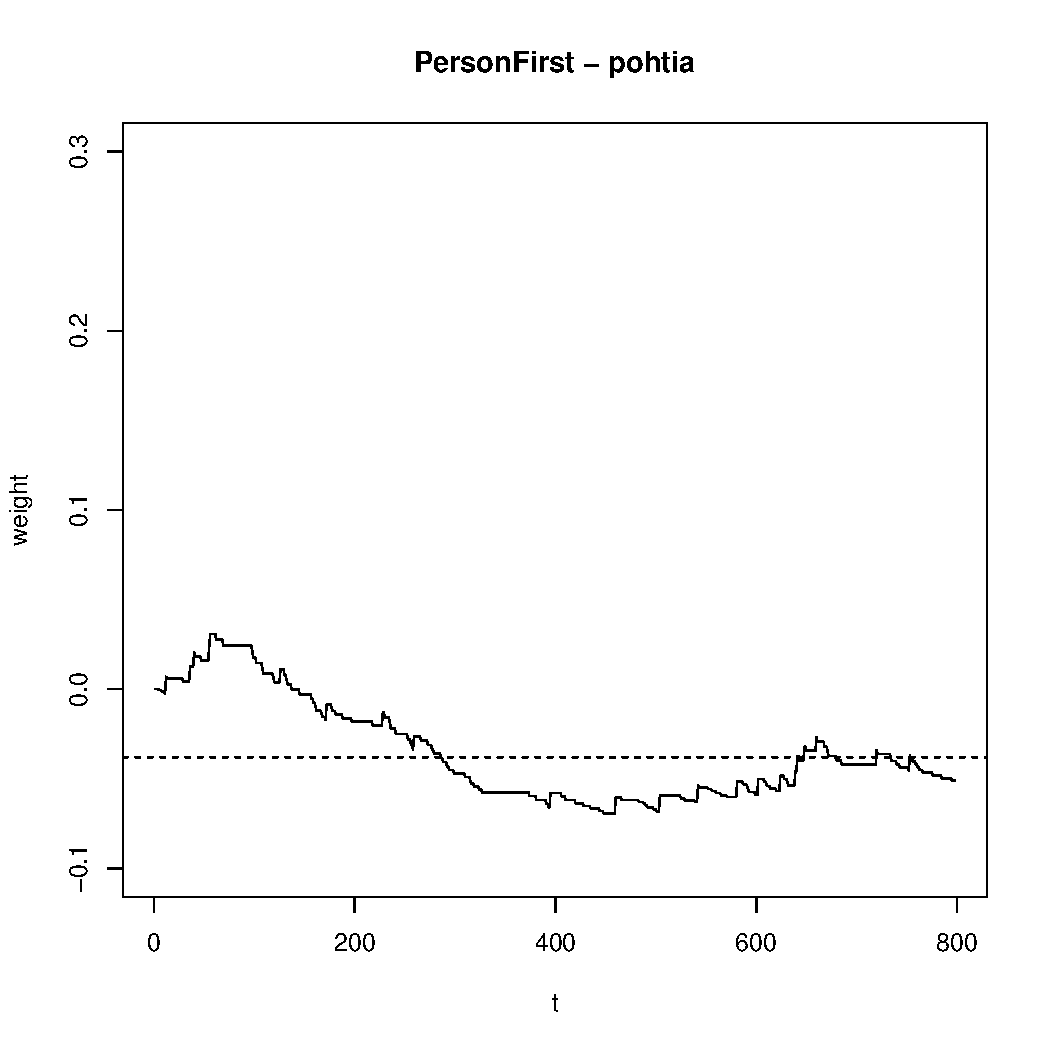
\includegraphics[width=8cm]{{{img/think.qitl1.PersonFirst_pohtia_RW_vs_D}}}
  
\end{frame}

\begin{frame}
\frametitle{QITL-01: Linguistic production vs. judgments}

{\scriptsize
\begin{table}[h]
\begin{tabular}{ c  c || c || c  c}
\hline
Forced-choice &               & Frequency  &               & Acceptability \\
Dispreferred  & Preferred     & (relative) & Unacceptable  & Acceptable  \\ \hline \hline
\multicolumn{1}{c|}{$\varnothing$} & +             & Frequent   & \multicolumn{1}{c|}{$\varnothing$} & +           \\ \hline
\multicolumn{1}{c|}{+}             & $\varnothing$ & Rare       & \multicolumn{1}{c|}{+}             & +           \\
\hline
\end{tabular}
\end{table}
}

      $Frequency \Rightarrow Acceptability$ \\
      $Unacceptability \Rightarrow Rarity$ \\
      $\neg(Acceptability \Rightarrow Frequency)$ \\
      $\neg(Rarity \Rightarrow Unacceptability)$ \\

\end{frame}

\begin{frame}
  \frametitle{QITL-01 through the lenses of QITL-6 (courtesy of Dagmar Divjak}

  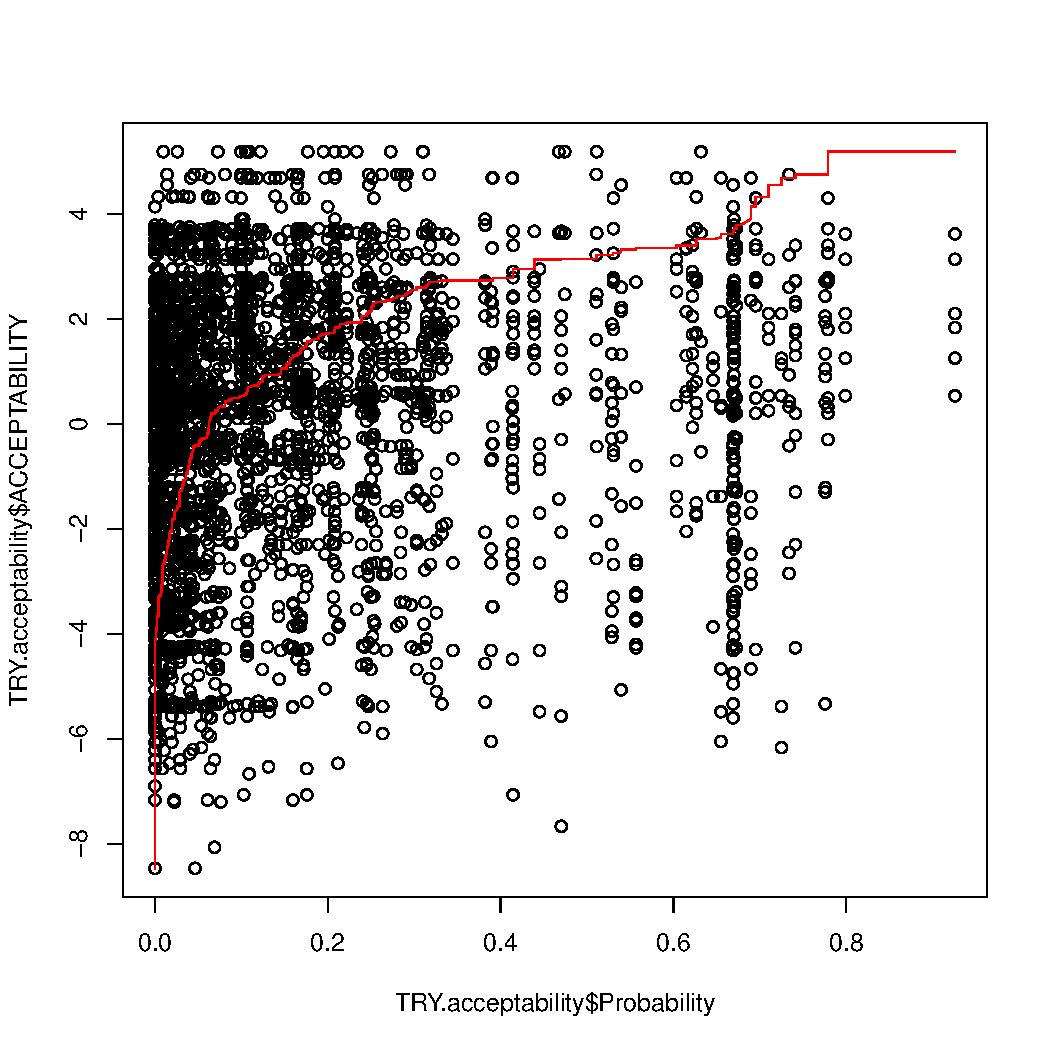
\includegraphics[width=7cm]{{{img/TRY.ACCEPTABILITY_vs_Probability}}}
  
\end{frame}

\begin{frame}
  \frametitle{Simple vs. complex settings - QITL-2 revisited}

  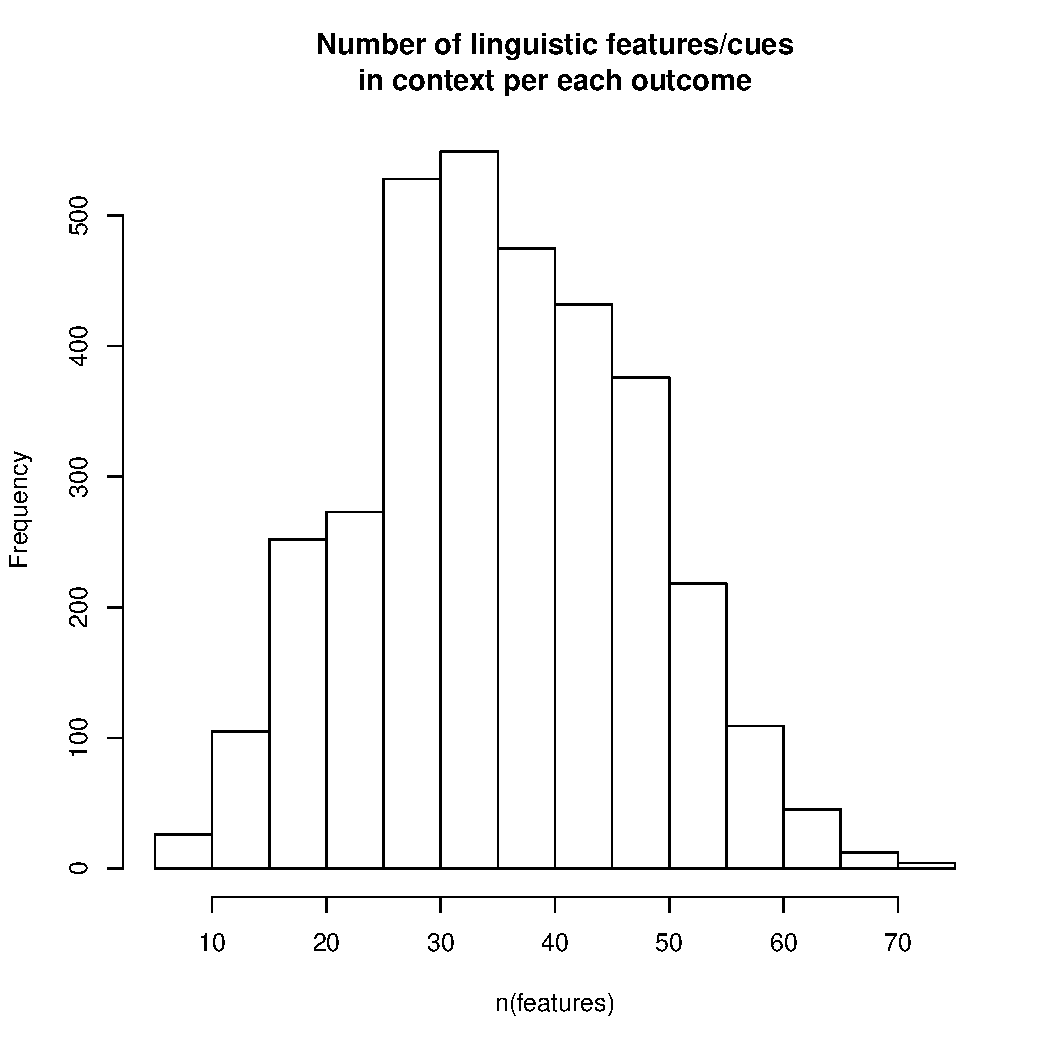
\includegraphics[width=8cm]{{{img/THINK.maximal_linguistic_variable_density}}}
  
\end{frame}

\begin{frame}
  \frametitle{QITL-1 through the lenses of NDL: 1/4}

  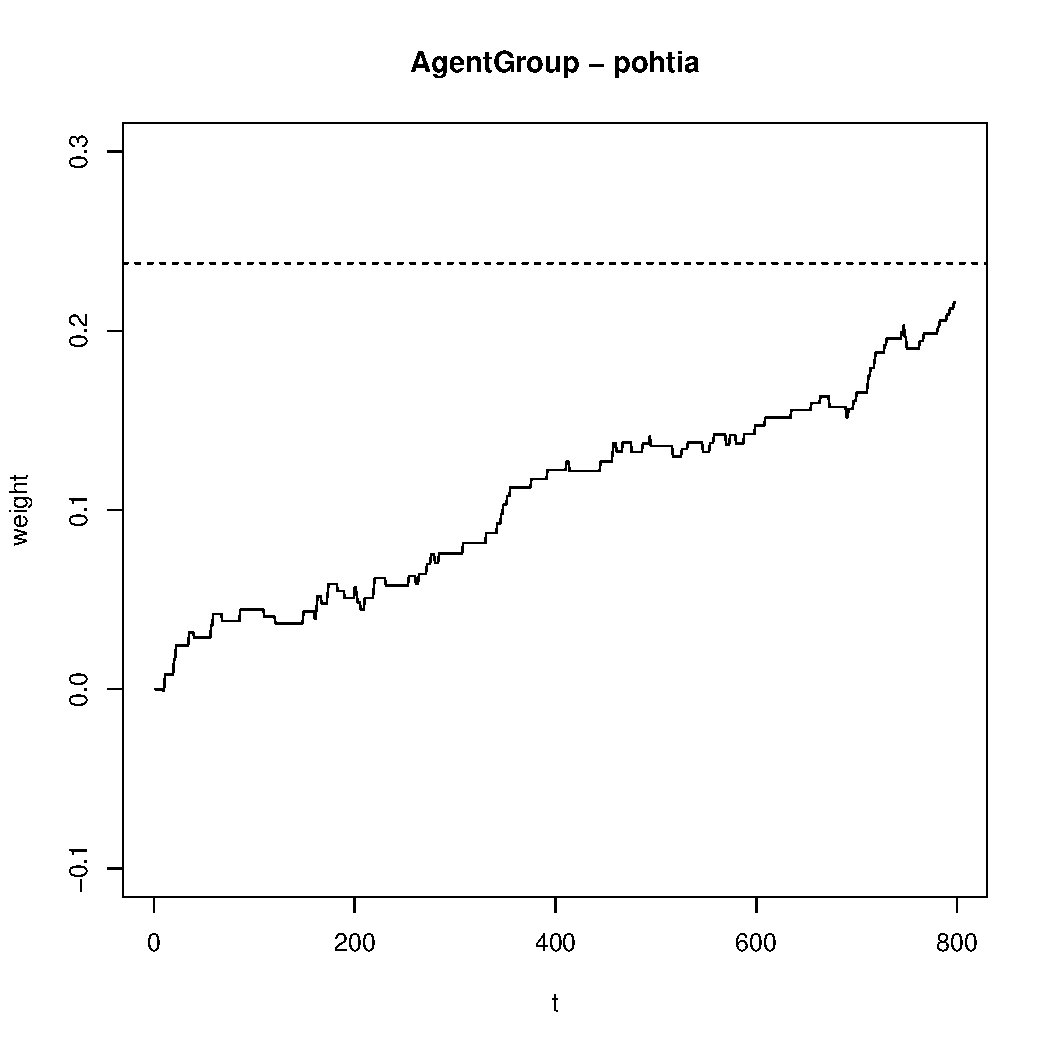
\includegraphics[width=8cm]{{{img/think.qitl1.AgentGroup_pohtia_RW_vs_D}}}
  
\end{frame}

\begin{frame}
\frametitle{QITL-4 revisited - comparison of NDL with statistical methods -- Classification Accuracy \& Recall}

% latex table generated in R 2.15.0 by xtable 1.7-0 package
% Thu May 24 17:10:59 2012
\begin{table}[ht]
\begin{center}
{\footnotesize
\begin{tabular}{lrrr}
  \hline
 & $\lambda_{\mbox{\tiny prediction}}$ & $\tau_{\mbox{\tiny classification}}$ & Accuracy \\ 
  \hline
Polytomous logistic regression & 0.447 & 0.516 & 0.646 \\ 
  (One-vs-rest) &  &  &  \\ 
  Polytomous mixed logistic regression &  &  &  \\ 
  (Poisson reformulation) &  &  &  \\ 
  1|Register & 0.435 & 0.505 & 0.638 \\ 
  1|Genre & 0.433 & 0.504 & 0.637 \\ 
  1|Lexeme & 0.428 & 0.499 & 0.634 \\ 
  1|Register + 1|Lexeme & 0.431 & 0.502 & 0.636 \\ 
  Support Vector Machine & 0.414 & 0.487 & 0.625 \\ 
  Memory-Based Learning & 0.287 & 0.376 & 0.543 \\ 
  (TiMBL) &  &  &  \\ 
  Random Forests & 0.445 & 0.515 & 0.645 \\ 
  Naive Discriminative Learning & 0.442 & 0.511 & 0.642 \\ 
   \hline
\end{tabular}
}
\caption{Classification diagnostics for five models fitted to the English data set ($n=909$).}
\label{tab:results}
\end{center}
\end{table}
\end{frame}

%%% Local Variables: 
%%% mode: latex
%%% TeX-master: "../qitl6_evert_arppe"
%%% End: 
